\section[Mandatory Access Control (MAC)]{Mandatory \\ Access Control (MAC)}
% --- Slide 45: Contents (Chuyển tiếp sang phần 3) ---
\begin{frame}{Contents}
    \Large
    \begin{enumerate}
        \color{gray} % Làm mờ các mục không phải hiện tại
        \item Introduction to Database Security Issues
        \item Discretionary Access Control (DAC)
        
        \color{black} \bfseries % Tô đen và in đậm mục hiện tại
        \item Mandatory Access Control (MAC)
        
        \color{gray} \mdseries % Quay lại màu xám và font thường
        \item Role-Based Access Control (RBAC)
        \item Attribute-Based Access Control (ABAC)
        \item Context-Based Access Control (CBAC)
    \end{enumerate}
\end{frame}

% --- Slide 46: Mandatory Access Control (Định nghĩa) ---
\begin{frame}{Mandatory Access Control}
    \Large
    \begin{itemize}
        \vspace{-1.5cm}
        \item Granting access to the data on the basis of \textbf{users' clearance level} and the \textbf{sensitivity level of the data}.
        
        \vspace{0.5cm}
        \item \textbf{Bell-LaPadula's two principles}:
        \begin{itemize}
            \large
            \item No read-up
            \item No write-down secrecy.
        \end{itemize}
    \end{itemize}
\end{frame}

% --- Slide 47: Bell-LaPadula Model ---
\begin{frame}{Bell-LaPadula Model}
    \Large
    \begin{itemize}
        \vspace{-0.5cm}
        \item Typical security classes are top secret (TS), secret (S), confidential (C), and unclassified (U), where TS is the highest level and U is the lowest one: 
        \[ TS \ge S \ge C \ge U \]
        
        \item Two restrictions are enforced on data access based on the subject/object classifications:
        \begin{enumerate}
            \large
            \item A subject S is not allowed \textbf{read access} to an object O unless \textbf{class(S) $\ge$ class(O)}. \\
            $\to$ This is known as the \textbf{simple security property}.
            
            \item A subject S is not allowed to \textbf{write} an object O unless \textbf{class(S) $\le$ class(O)}. \\
            $\to$ This known as the \textbf{star property} (or \textbf{* property}).
        \end{enumerate}
    \end{itemize}
\end{frame}
% --- ĐỊNH NGHĨA KIỂU HÌNH VẼ CHUNG (Cho gọn code) ---
\tikzset{
    mac_node/.style={font=\small},
    mac_user/.style={mac_node, circle, draw=black, thick, minimum size=1.2cm, align=center, fill=white},
    mac_file/.style={mac_node, rectangle, draw=black, thick, minimum width=2cm, minimum height=1.2cm, align=center, fill=white},
    mac_pgm/.style={mac_node, rectangle, draw=black, thick, minimum width=1.5cm, minimum height=2.2cm, align=center, fill=white},
    mac_th/.style={mac_node, rectangle, draw=black, thick, fill=white, minimum size=0.6cm, inner sep=1pt},
    mac_arrow/.style={->, >=stealth, thick}
}

% --- Slide 48: Why star property? (Setup) ---
\begin{frame}{Why star property?}
    \centering
    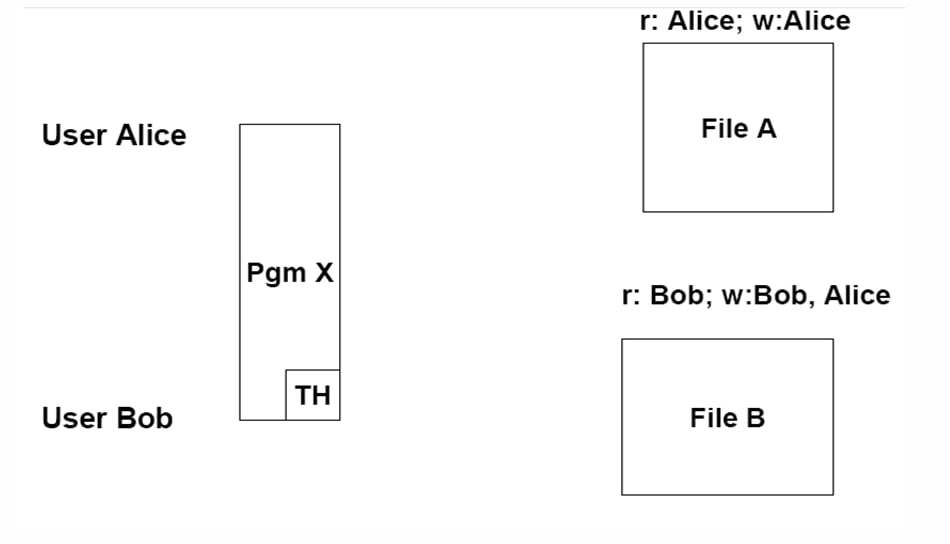
\includegraphics[width=0.9\textwidth ]{Assets/trojanhorse2.jpg}

\end{frame}


% --- Slide 49: Why star property? (Cuộc tấn công) ---
\begin{frame}{Why star property?}
    \centering
    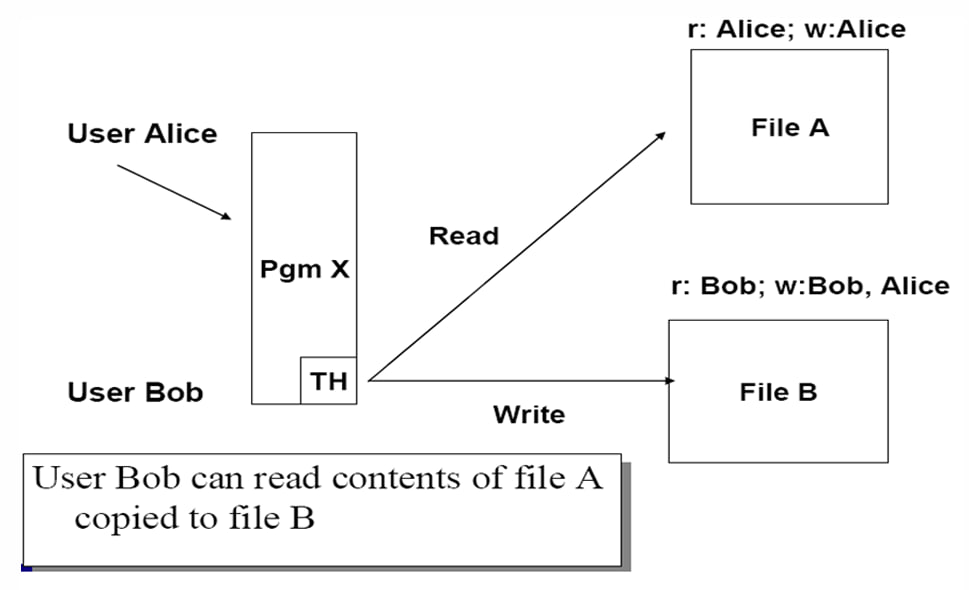
\includegraphics[width = 0.85\textwidth]{Assets/trojanhorse3.jpg}
\end{frame}

% --- Slide 50: Why star property? (Ngăn chặn bằng Star Property) ---
\begin{frame}{Why star property?}
    \centering
    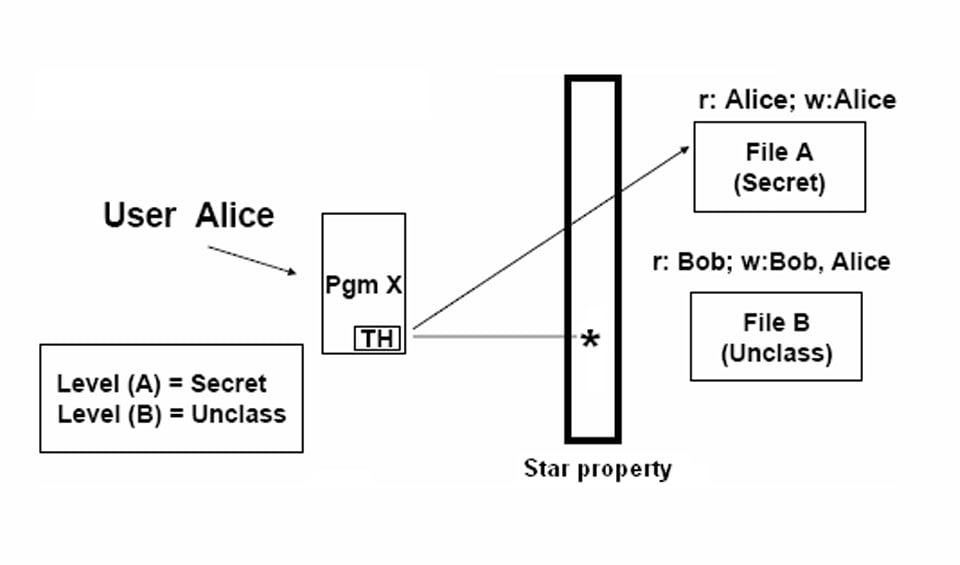
\includegraphics[width = 0.9\textwidth]{Assets/trojanhorse4.jpg}
\end{frame}

% --- Slide 51: Multilevel relation (1) ---
\begin{frame}{Multilevel relation (1)}
    \large % Giảm từ \Large xuống \large để tổng thể gọn hơn
    \begin{itemize}
        \setlength{\itemsep}{0.25cm} % Ép khoảng cách giữa các gạch đầu dòng lại
        \vspace{-0.5cm} % Kéo toàn bộ text lên trên một chút
        
        \item \textbf{Multilevel relation}: MAC + relational database model.
        
        \item \textbf{Data objects}: attributes and tuples.
        
        \item Each attribute A is associated with a \textbf{classification attribute C}.
        
        \item A \textbf{tuple classification attribute TC} is to provide a classification for each tuple as a whole, the highest of all attribute classification values.
        
        % Công thức toán học (đã bỏ vspace thừa để tiết kiệm diện tích)
        \[ R(A_{1},C_{1},A_{2},C_{2},...,A_{n},C_{n},TC) \]
        
        \item The \textbf{apparent key} of a multilevel relation is the set of attributes that would have formed the primary key in a regular (single-level) relation.
    \end{itemize}
\end{frame}

% --- Slide 52: Multilevel relation (2) ---
\begin{frame}{Multilevel relation (2)}
    \Large
    \textbf{EMPLOYEE}
    \vspace{0.05cm}
    
    % Bảng dữ liệu gốc (Hiển thị đầy đủ thông tin kèm nhãn bảo mật)
    \begin{center}
    \resizebox{0.8\textwidth}{!}{
        \begin{tabular}{|l|l|l|c|}
            \hline
            \rowcolor{gray!20} \textbf{Name} & \textbf{Salary} & \textbf{Job Performance} & \textbf{TC} \\
            \hline
            Smith \textbf{U} & 40000 \textbf{C} & Fair \textbf{S} & \textbf{S} \\
            \hline
            Brown \textbf{C} & 80000 \textbf{S} & Good \textbf{C} & \textbf{S} \\
            \hline
        \end{tabular}
    }
    \end{center}
    \small \textit{(U: Unclassified, C: Confidential, S: Secret)}
    
    \vspace{0.25cm}
    \begin{itemize}
      \large  \item A multilevel relation will appear to contain \textbf{different data} to subjects (users) with \textbf{different security levels}.
    \end{itemize}
\end{frame}


% --- Slide 53: Multilevel relation (3) ---
\begin{frame}{Multilevel relation (3)}
    \Large
    % Câu lệnh SQL theo format chuẩn của bài
    \texttt{\textbf{SELECT * FROM EMPLOYEE}}
    
    \vspace{0.2cm}
    \normalsize \textbf{EMPLOYEE}:
    
    % BẢNG 1 (Bảng gốc)
    \begin{center}
    \vspace{-0.2cm}
    \resizebox{0.7\textwidth}{!}{
        \begin{tabular}{|l|l|l|c|}
            \hline
            \rowcolor{gray!20} \textbf{Name} & \textbf{Salary} & \textbf{JobPerformance} & \textbf{TC} \\
            \hline
            Smith \textbf{U} & 40000 \textbf{C} & Fair \textbf{S} & \textbf{S} \\
            \hline
            Brown \textbf{C} & 80000 \textbf{S} & Good \textbf{C} & \textbf{S} \\
            \hline
        \end{tabular}
    }
    \end{center}
    
    \vspace{0.1cm}
    \begin{itemize}
       \large \item View for a user with security level \textbf{S} (Secret):
    \end{itemize}
    
    % BẢNG 2 (Góc nhìn của User S)
    \begin{center}
    \vspace{-0.2cm}
    \resizebox{0.7\textwidth}{!}{
        \begin{tabular}{|l|l|l|c|}
            \hline
            \rowcolor{gray!20} \textbf{Name} & \textbf{Salary} & \textbf{JobPerformance} & \textbf{TC} \\
            \hline
            Smith \textbf{U} & 40000 \textbf{C} & Fair \textbf{S} & \textbf{S} \\
            \hline
            Brown \textbf{C} & 80000 \textbf{S} & Good \textbf{C} & \textbf{S} \\
            \hline
        \end{tabular}
    }
    \end{center}
\end{frame}

% --- Slide 54: Multilevel relation (4) - User Level C ---
\begin{frame}{Multilevel relation (4)}
    \Large
    % Câu lệnh SQL theo format chuẩn
    \texttt{\textbf{SELECT * FROM EMPLOYEE}}
    
    \vspace{0.2cm}
    \normalsize \textbf{EMPLOYEE} table:
    
    % BẢNG 1 (Bảng gốc)
    \begin{center}
    \vspace{-0.2cm}
    \resizebox{0.7\textwidth}{!}{
        \begin{tabular}{|l|l|l|c|}
            \hline
            \rowcolor{gray!20} \textbf{Name} & \textbf{Salary} & \textbf{JobPerformance} & \textbf{TC} \\
            \hline
            Smith \textbf{U} & 40000 \textbf{C} & Fair \textbf{S} & \textbf{S} \\
            \hline
            Brown \textbf{C} & 80000 \textbf{S} & Good \textbf{C} & \textbf{S} \\
            \hline
        \end{tabular}
    }
    \end{center}
    
    \vspace{0.2cm}
    \begin{itemize}
        % Dùng \large để tăng cỡ chữ dòng này lên một chút theo yêu cầu
        \large \item View for a user with security level \textbf{C} (Confidential):
    \end{itemize}
    
    % BẢNG 2 (Góc nhìn của User C)
    \begin{center}
    \vspace{-0.2cm}
    \resizebox{0.7\textwidth}{!}{
        \begin{tabular}{|l|l|l|c|}
            \hline
            \rowcolor{gray!20} \textbf{Name} & \textbf{Salary} & \textbf{JobPerformance} & \textbf{TC} \\
            \hline
            Smith \textbf{U} & 40000 \textbf{C} & NULL \textbf{C} & \textbf{C} \\
            \hline
            Brown \textbf{C} & NULL \textbf{C} & Good \textbf{C} & \textbf{C} \\
            \hline
        \end{tabular}
    }
    \end{center}
\end{frame}


% --- Slide 55: Multilevel relation (5) - User Level U ---
% --- Slide 55: Multilevel relation (5) - User Level U ---
\begin{frame}{Multilevel relation (5)}
    \Large
    % Câu lệnh SQL theo format chuẩn
    \texttt{\textbf{SELECT * FROM EMPLOYEE}}
    
    \vspace{0.2cm}
    \normalsize \textbf{EMPLOYEE} table:
    
    % BẢNG 1 (Bảng gốc)
    \begin{center}
    \vspace{-0.2cm}
    \resizebox{0.7\textwidth}{!}{
        \begin{tabular}{|l|l|l|c|}
            \hline
            \rowcolor{gray!20} \textbf{Name} & \textbf{Salary} & \textbf{JobPerformance} & \textbf{TC} \\
            \hline
            Smith \textbf{U} & 40000 \textbf{C} & Fair \textbf{S} & \textbf{S} \\
            \hline
            Brown \textbf{C} & 80000 \textbf{S} & Good \textbf{C} & \textbf{S} \\
            \hline
        \end{tabular}
    }
    \end{center}
    
    \vspace{0.2cm}
    \begin{itemize}
        % Dùng \large để làm nổi bật sự chuyển đổi góc nhìn
        \large \item View for a user with security level \textbf{U} (Unclassified):
    \end{itemize}
    
    % BẢNG 2 (Góc nhìn của User U - Dòng Brown bị ẩn hoàn toàn)
    \begin{center}
    \vspace{-0.2cm}
    \resizebox{0.7\textwidth}{!}{
        \begin{tabular}{|l|l|l|c|}
            \hline
            \rowcolor{gray!20} \textbf{Name} & \textbf{Salary} & \textbf{JobPerformance} & \textbf{TC} \\
            \hline
            Smith \textbf{U} & NULL \textbf{U} & NULL \textbf{U} & \textbf{U} \\
            \hline
        \end{tabular}
    }
    \end{center}
\end{frame}

% --- Slide 56: Properties of Multilevel relation (1) ---
\begin{frame}{Properties of Multilevel relation (1)}
    \Large
    \begin{itemize}
        \vspace{-1.5cm}
        \item \textbf{Read and write operations}: satisfy the:
        
        \vspace{0.5cm}
        \begin{itemize}
            \large
            \setlength{\itemsep}{0.3cm}
            \item \textbf{No Read-Up} principle.
            \item \textbf{No Write-Down} principle.
        \end{itemize}
        
    \end{itemize}
\end{frame}

% --- Slide 57: Properties of Multilevel relation (2) ---
\begin{frame}{Properties of Multilevel relation (2)}
    \Large
    \begin{itemize}
        \vspace{-1cm}
        \item \textbf{Entity integrity}: all attributes that are members of the \textbf{apparent key} must not be null and must have the \textbf{same security classification} within each individual tuple.
        
        \vspace{0.3cm}
        \item In addition, all other attribute values in the tuple must have a security classification \textbf{greater than or equal to} that of the apparent key.
        
        \vspace{0.3cm}
        \item This constraint ensures that a user can see the key if the user is permitted to see any part of the tuple at all.
    \end{itemize}
\end{frame}

% --- Slide 58: Properties of Multilevel relation (3) ---
\begin{frame}{Properties of Multilevel relation (3)}
    \Large
    \begin{itemize}
        \vspace{-1.5cm}
        \item \textbf{Polyinstantiation}: where several tuples can have the \textbf{same apparent key value} but have \textbf{different attribute values} for users at different classification levels.
    \end{itemize}
\end{frame}

% --- Slide 59: Polyinstantiation example (1) ---
\begin{frame}{Polyinstantiation example (1)}
    \vspace{0.2cm}
    \normalsize \textbf{EMPLOYEE}
    
    % BẢNG 1 (Bảng gốc)
    \begin{center}
    \vspace{-0.2cm}
    \resizebox{0.7\textwidth}{!}{
        \begin{tabular}{|l|l|l|c|}
            \hline
            \rowcolor{gray!20} \textbf{Name} & \textbf{Salary} & \textbf{JobPerformance} & \textbf{TC} \\
            \hline
            Smith \textbf{U} & 40000 \textbf{C} & Fair \textbf{S} & \textbf{S} \\
            \hline
            Brown \textbf{C} & 80000 \textbf{S} & Good \textbf{C} & \textbf{S} \\
            \hline
        \end{tabular}
    }
    \end{center}
    
    \vspace{0.2cm}
    \begin{itemize}
        % Dùng \large để làm nổi bật dòng này
        \large \item A user with security level \textbf{C}:
    \end{itemize}
    
    \vspace{0.1cm}
    \normalsize \textbf{EMPLOYEE}
    
    % BẢNG 2 (Góc nhìn của User C)
    \begin{center}
    \vspace{-0.2cm}
    \resizebox{0.7\textwidth}{!}{
        \begin{tabular}{|l|l|l|c|}
            \hline
            \rowcolor{gray!20} \textbf{Name} & \textbf{Salary} & \textbf{JobPerformance} & \textbf{TC} \\
            \hline
            Smith \textbf{U} & 40000 \textbf{C} & NULL \textbf{C} & \textbf{C} \\
            \hline
            Brown \textbf{C} & NULL \textbf{C} & Good \textbf{C} & \textbf{C} \\
            \hline
        \end{tabular}
    }
    \end{center}
    \small (Values with higher security level are shown as NULL)
\end{frame}


% --- Slide 60: Polyinstantiation example (2) ---
\begin{frame}{Polyinstantiation example (2)}
    \large % Hạ cỡ chữ tổng thể xuống một chút để nội dung nằm gọn trong slide
    \begin{itemize}
        \item A user with security level \textbf{C} executes:
    \end{itemize}
    
    \vspace{0.1cm}
    % Bọc lệnh SQL vào flushleft để ngắt dòng chuẩn xác và tiết kiệm không gian
    \begin{flushleft}
        \ttfamily \textbf{UPDATE} EMPLOYEE \\
        \textbf{SET} Job\_performance = 'Excellent' \\
        \textbf{WHERE} Name = 'Smith';
    \end{flushleft}
    
    \vspace{0.03cm}
    \textbf{Resulting Table (Polyinstantiation occurs):}
    
    \begin{center}
    \vspace{-0.2cm} % Kéo bảng lên sát chữ
    \resizebox{0.7\textwidth}{!}{ % Ép lại 0.7 cho đồng bộ với các slide trước
        \begin{tabular}{|l|l|l|c|}
            \hline
            \rowcolor{gray!20} \textbf{Name} & \textbf{Salary} & \textbf{JobPerformance} & \textbf{TC} \\
            \hline
            Smith \textbf{U} & 40000 \textbf{C} & Fair \textbf{S} & \textbf{S} \\
            \hline
            % Dòng mới sinh ra được tô màu vàng nhạt để làm nổi bật
            \rowcolor{yellow!30} Smith \textbf{U} & 40000 \textbf{C} & Excellent \textbf{C} & \textbf{C} \\
            \hline
            Brown \textbf{C} & 80000 \textbf{S} & Good \textbf{C} & \textbf{S} \\
            \hline
        \end{tabular}
    }
    \end{center}
    
    \vspace{0.05cm}
    \centering \normalsize \textbf{Polyinstantiation of the Smith tuple.}
\end{frame}

% --- Slide: Polyinstantiation example (3) - Lệnh INSERT ---
\begin{frame}{Polyinstantiation example (3)}
    \large
    \vspace{-0.05cm}
    \begin{itemize}
        \item A user with security level \textbf{U} (Unclassified) executes:
    \end{itemize}
    
    \vspace{0.05cm}
    \begin{flushleft}
        \ttfamily \textbf{INSERT INTO} EMPLOYEE \\
        \textbf{VALUES} ('Brown', 50000, 'Average');
    \end{flushleft}
    
    \vspace{0.03cm}
    \textbf{Resulting Table (Polyinstantiation occurs):}
    
    \begin{center}
    \vspace{-0.2cm}
    \resizebox{0.85\textwidth}{!}{
        \begin{tabular}{|l|l|l|c|}
            \hline
            \rowcolor{gray!20} \textbf{Name} & \textbf{Salary} & \textbf{JobPerformance} & \textbf{TC} \\
            \hline
            % Dòng mới sinh ra do U insert
            \rowcolor{yellow!30} Brown \textbf{U} & 50000 \textbf{U} & Average \textbf{U} & \textbf{U} \\
            \hline
            % Dòng gốc của S (U không nhìn thấy)
            Brown \textbf{C} & 80000 \textbf{S} & Good \textbf{C} & \textbf{S} \\
            \hline
        \end{tabular}
    }
    \end{center}
    
    \vspace{0.01cm}
    \begin{itemize}
        \normalsize
        \item If the DBMS rejects the INSERT, the \textbf{U} user would deduce that 'Brown' exists at a higher level (Information Leak!).
        \item Allowing it closes this \textbf{covert channel}.
    \end{itemize}
\end{frame}

% --- Slide 62: Polyinstantiation example (4) - Lệnh DELETE ---
\begin{frame}{Polyinstantiation example (4)}
    \large
    \begin{itemize}
        \item Continuing from the previous state, a user with security level \textbf{U} executes:
    \end{itemize}
    
    \vspace{0.2cm}
    \begin{flushleft}
        \ttfamily \textbf{DELETE FROM} EMPLOYEE \\
        \textbf{WHERE} Name = 'Brown';
    \end{flushleft}
    
    \vspace{0.2cm}
    \textbf{Resulting Table:}
    
    \begin{center}
    \vspace{-0.2cm}
    \resizebox{0.85\textwidth}{!}{
        \begin{tabular}{|l|l|l|c|}
            \hline
            \rowcolor{gray!20} \textbf{Name} & \textbf{Salary} & \textbf{JobPerformance} & \textbf{TC} \\
            \hline
            % Dòng gốc của S (Vẫn an toàn)
            \rowcolor{green!10} Brown \textbf{C} & 80000 \textbf{S} & Good \textbf{C} & \textbf{S} \\
            \hline
        \end{tabular}
    }
    \end{center}
    \small \centering \textit{(The U-level 'Brown' tuple is deleted, but the higher-level tuple survives)}
    
    \vspace{0.05cm}
    \begin{itemize}
        \normalsize
        \item The DBMS \textbf{only deletes the tuple visible at level U}.
        \item \textbf{Conclusion:} Lower-level subjects cannot destroy or modify objects they do not have clearance to access (prevents sabotage).
    \end{itemize}
\end{frame}



% --- Slide 61: Comparing DAC and MAC (1) ---
\begin{frame}{Comparing DAC and MAC (1)}
    \Large
    \begin{itemize}
        \item \textbf{Discretionary Access Control (DAC)} policies are characterized by a \textbf{high degree of flexibility}, which makes them suitable for a large variety of application domains.
        
        \vspace{0.3cm} 
        % Bắt đầu Level 2
        \begin{itemize}
            \large % Hạ cỡ chữ xuống 1 cấp cho chuẩn Level 2
            \item The \textbf{main drawback} of DAC models is their \textbf{vulnerability to malicious attacks}, such as \textbf{Trojan horses} embedded in application programs.
        \end{itemize}
    \end{itemize}
\end{frame}


% --- Slide 62: Comparing DAC and MAC (2) ---
\begin{frame}{Comparing DAC and MAC (2)}
    \Large
    \begin{itemize}
        \item By contrast, \textbf{mandatory policies} ensure a \textbf{high degree of protection} in a way, they prevent any illegal flow of information.
        
        \vspace{0.3cm}
        \item Mandatory policies have the drawback of being \textbf{too rigid} and they are only applicable in \textbf{limited environments}.
        
        \vspace{0.3cm}
        \item In many practical situations, \textbf{discretionary policies are preferred} because they offer a better \textbf{trade-off} between security and applicability.
    \end{itemize}
\end{frame}